% `template.tex', a bare-bones example employing the AIAA class.
%
% For a more advanced example that makes use of several third-party
% LaTeX packages, see `advanced_example.tex', but please read the
% Known Problems section of the users manual first.
%
% Typical processing for PostScript (PS) output:
%
%  latex template
%  latex template   (repeat as needed to resolve references)
%
%  xdvi template    (onscreen draft display)
%  dvips template   (postscript)
%  gv template.ps   (onscreen display)
%  lpr template.ps  (hardcopy)
%
% With the above, only Encapsulated PostScript (EPS) images can be used.
%
% Typical processing for Portable Document Format (PDF) output:
%
%  pdflatex template
%  pdflatex template      (repeat as needed to resolve references)
%
%  acroread template.pdf  (onscreen display)
%
% If you have EPS figures, you will need to use the epstopdf script
% to convert them to PDF because PDF is a limmited subset of EPS.
% pdflatex accepts a variety of other image formats such as JPG, TIF,
% PNG, and so forth -- check the documentation for your version.
%
% If you do *not* specify suffixes when using the graphicx package's
% \includegraphics command, latex and pdflatex will automatically select
% the appropriate figure format from those available.  This allows you
% to produce PS and PDF output from the same LaTeX source file.
%
% To generate a large format (e.g., 11"x17") PostScript copy for editing
% purposes, use
%
%  dvips -x 1467 -O -0.65in,0.85in -t tabloid template
%
% For further details and support, read the Users Manual, aiaa.pdf.


% Try to reduce the number of latex support calls from people who
% don't read the included documentation.
%


\typeout{}\typeout{If latex fails to find aiaa-tc, read the README file!}
%


\documentclass[]{aiaa-tc}% insert '[draft]' option to show overfull boxes
\usepackage{float}
\usepackage{epstopdf}

\title{GPS Navigation in a Visibility Challenged Environment}

\author{
	Ryan D. Riveland and Johnathan Clouse%
	\thanks{Graduate Students, Aerospace Engineering Sciences, 1111 Engineering Drive, Boulder, CO, 80309-0429}\\
	{\normalsize\itshape
		University of Colorado, Boulder, CO, 80309-0429, USA}
}

% Define commands to assure consistent treatment throughout document
\newcommand{\eqnref}[1]{(\ref{#1})}
\newcommand{\class}[1]{\texttt{#1}}
\newcommand{\package}[1]{\texttt{#1}}
\newcommand{\file}[1]{\texttt{#1}}
\newcommand{\BibTeX}{\textsc{Bib}\TeX}

\usepackage[euler]{textgreek}
\usepackage[colorlinks=true]{hyperref}
\hypersetup{urlcolor=cyan}

\usepackage{listings}
\usepackage{color} %red, green, blue, yellow, cyan, magenta, black, white
\definecolor{mygreen}{RGB}{28,172,0} % color values Red, Green, Blue
\definecolor{mylilas}{RGB}{170,55,241}

\usepackage{tablefootnote}
\usepackage{graphicx}
\usepackage{amsmath}
\usepackage{bm}
\usepackage{subfigure}

\definecolor{mylilas}{RGB}{170,55,241}

% See p.105 of "TeX Unbound" for suggested values.
% See pp. 199-200 of Lamport's "LaTeX" book for details.
%   General parameters, for ALL pages:
\renewcommand{\topfraction}{0.9}	% max fraction of floats at top
\renewcommand{\bottomfraction}{0.8}	% max fraction of floats at bottom
%   Parameters for TEXT pages (not float pages):
\setcounter{topnumber}{2}
\setcounter{bottomnumber}{2}
\setcounter{totalnumber}{4}     % 2 may work better
\setcounter{dbltopnumber}{2}    % for 2-column pages
\renewcommand{\dbltopfraction}{0.9}	% fit big float above 2-col. text
\renewcommand{\textfraction}{0.07}	% allow minimal text w. figs
%   Parameters for FLOAT pages (not text pages):
\renewcommand{\floatpagefraction}{0.7}	% require fuller float pages
% N.B.: floatpagefraction MUST be less than topfraction !!
\renewcommand{\dblfloatpagefraction}{0.7}	% require
    \makeatletter
    \renewcommand\l@section{\@dottedtocline{2}{1.5em}{3em}}
    \makeatother
    
\begin{document}
	

	
	\maketitle
	
	\begin{abstract}
		\noindent The purpose of this experiment was to investigate the accuracy of a hand-held GPS receiver in an environment where signal visibility was limited. A route was chosen west of Castle Rock, CO where the first section was expected to have ample signal availability. The second section was in a canyon where signal availability was expected to be limited due to terrain. As expected, position error in the second section was degraded relative to the first section. It was concluded that terrain has a strong influence on GPS navigation accuracy.
		
	\end{abstract}
	
	\newpage
	
	\tableofcontents
	
	\newpage
	
	\section{Objectives}
	
	\noindent The objective of this experiment was to investigate how varying terrain would impact the ability to navigate using GPS. In mountainous regions, signal visibility may be obstructed by the terrain leading to potential dilution of precision (DOP) of the solution. Several factors contributed to the extent to which the GPS signals may be obstructed. A few of these factors were the height of the terrain relative to the user, time of day, and latitude. The experiment attempted to account for all of these factors in the results. 
	
	\vspace{5 mm}
	
	\noindent Since two hand-held GPS receivers were available, the Wide Area Augmentation System (WAAS) capability on one of the receivers was turned off to determine if using WAAS could mitigate navigation difficulties due to limited signal availability from the nominal GPS constellation. WAAS is a GPS augmentation system completed in 2003 by the FAA\cite{Misra:2012}. 
	
	\vspace{5 mm}
	
	\noindent The results of this experiment are of interest to those that may want to rely on GPS navigation for mountain recreation, to include hiking or any off road recreation. It was hypothesized that GPS navigation would be more accurate in wide-open terrain where more GPS signals were available for processing. Additionally, it was expected that the WAAS-enabled GPS receiver would be more accurate and precise than the GPS receiver where WAAS had been disabled.
	
	\section{Method}
	
	\noindent A 15-mile route along US Highway 85/ CO State Highway 67 west of Castle Rock, CO was chosen due to its wide variety of terrain. The first section of the route was wide-open with low elevation terrain. Signal availability was expected to be ample in this area. The second section was in a Rocky Mountain canyon where signal availability was expected to be limited due to the higher terrain. During the experiment, GPS tracks were recorded using both a Garmin GPS60 and a Delorme Earthmate PN-40. For consistency, both receivers were set to collect track points at 1 second intervals (which was also the fastest they could record).
	
	\vspace{5 mm}
	
	\noindent While driving the route, azimuth and elevation measurements were taken of the terrain at various waypoints. Every effort was made to choose waypoints with varying terrain, however safe turn-off locations were limited. The azimuth measurements were taken using a compass and the elevation was measured using a clinometer at 45 degree azimuth intervals. In order to account for azimuth directions without measurements, the elevation was linearly interpolated between measurements. Digital photos of the signal strength screen were taken at each waypoint to correlate the signal strength vs. the visibility.
	
	\vspace{5 mm}
	
	\noindent At each waypoint the time, latitude, longitude, and height were extracted from the waypoint file output from the receiver. These data points were used to compute PRN azimuth and elevation. The azimuth and elevation points were plotted along with the linearly interpolated horizon mask to determine which PRN signals were actually available for navigation processing. 
	
	\vspace{5 mm} 
	
	\noindent To determine the accuracy of the position measurements, the tracks from each receiver were output to a .gpx file. This file is a standardized format recognized by a variety of GPS visualization software. For this experiment Google Earth was used for visualization. The highway on the Google Earth maps was used for qualitative truth. In addition to the position-performance truth, the visualization was used as a qualitative comparison between relative receiver performance. 
	
	\vspace{5 mm}
	
	\noindent In addition to qualitative comparisons, a few quantitative techniques were used to determine accuracy. Built into Google Earth, is a ruler tool that allowed the user to determine the distance between two points on a map. For this experiment, the road on the map was considered the truth. To determine position accuracy at various points, the distance could be measured between the superimposed track and the road. Secondly, data could be extracted from the .gpx files to determine the relative accuracy between the two receivers. The relative difference and root sum square (RSS) of latitude and longitude could be computed and plotted. 
	
	\vspace{5 mm}
	
	\noindent At the end of the route, the tracks were reset and data was collected along the path to the starting location using the same route. Because of this, and the redundancy of using two different receivers, only one trial was conducted. 
	
	\section{Experiment}
	
	\vspace{5 mm}
	
	\noindent The experiment was conducted on the afternoon of October 4, 2014. The weather conditions were sunny with a light wind. Since the method of travel was via car, the GPS receivers were set on the dashboard. Ideally, the GPS receivers would be held with the antenna facing upwards but this was not possible for safety reasons. As expected, locations to stop and collect horizon mask data were limited but every effort was made to take these measurements in locations with varying terrain. All other data collection activities were performed successfully.
	
	\section{Data and Results}
	
	\noindent The resulting GPS data from the trip were post-processed to find the relative error between the two receivers. The relative errors were plotted with waypoint information so that they could be cross referenced with the topographic elevation measurements. The relative error between the receivers can be seen in Figure~\ref{fig:Trip1Err} and Figure~\ref{fig:Trip2Err}. The tabular topographic measurements are shown in Table~\ref{t:WaypointsHorMask}. 
	
	\begin{figure}[H]
		\centering
		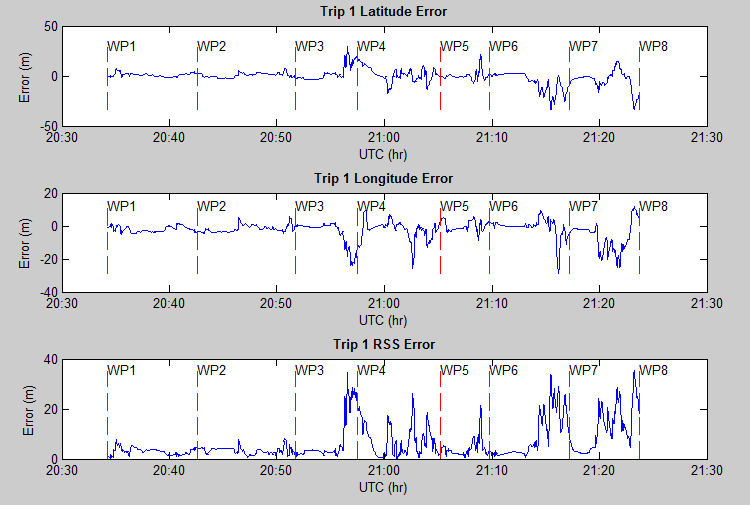
\includegraphics[width = 13cm]{Trip1Err.PNG}
		\caption{Relative receiver error observed during trip 1. }
		\label{fig:Trip1Err}
	\end{figure}
	
	\begin{figure}[H]
		\centering
		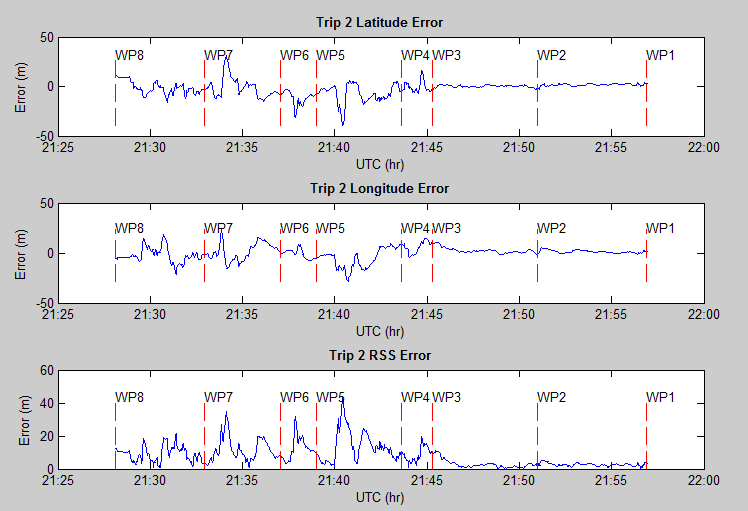
\includegraphics[width = 13cm]{Trip2Err.PNG}
		\caption{Relative receiver error observed during trip 2. }
		\label{fig:Trip2Err}
	\end{figure}
		
	\begin{table}[H]% no placement specified: defaults to here, top, bottom, page
		\begin{center}
			\caption{Horizon mask for all waypoints.}
			\label{t:WaypointsHorMask}
			\begin{tabular}{c|c|c|c|c|c|c|c|c}
				Az. & El. WP1 & El. WP2 & El. WP3& El. WP4 & El. WP5 & El. WP6 & El. WP7 & El. WP8\\ \hline
				0$^{\circ}$  & 5$^{\circ}$ & 2$^{\circ}$ & 9$^{\circ}$ & 18$^{\circ}$ & 8$^{\circ}$& 11 $^{\circ}$& 21$^{\circ}$& 12$^{\circ}$ \\
				45$^{\circ}$ & 4$^{\circ}$ & 0$^{\circ}$ & 1$^{\circ}$ & 24$^{\circ}$ & 3$^{\circ}$& 9$^{\circ}$& 15$^{\circ}$& 6$^{\circ}$ \\
				90$^{\circ}$ & 15$^{\circ}$ & 3$^{\circ}$ & 0$^{\circ}$ & 23$^{\circ}$ & 0$^{\circ}$& 3$^{\circ}$& 8$^{\circ}$& 7$^{\circ}$ \\
				135$^{\circ}$ & 3$^{\circ}$ & 6$^{\circ}$ & 0$^{\circ}$ & 13$^{\circ}$ & 0$^{\circ}$& 6$^{\circ}$& 6$^{\circ}$& 13$^{\circ}$ \\
				180$^{\circ}$ & 7$^{\circ}$ & 5$^{\circ}$ & 2$^{\circ}$ &  20$^{\circ}$ & 3$^{\circ}$& 7$^{\circ}$& 14$^{\circ}$& 6$^{\circ}$ \\
				225$^{\circ}$ & 3$^{\circ}$ & 3$^{\circ}$ & 15$^{\circ}$ & 26$^{\circ}$ & 3$^{\circ}$& 4$^{\circ}$& 7$^{\circ}$& 10$^{\circ}$ \\
				270$^{\circ}$ & 2$^{\circ}$ & 4$^{\circ}$ & 20$^{\circ}$ & 23$^{\circ}$ & 6$^{\circ}$& 9$^{\circ}$& 6$^{\circ}$& 11$^{\circ}$ \\
				315$^{\circ}$ & 2$^{\circ}$ & 3$^{\circ}$ & 10$^{\circ}$ & 15$^{\circ}$ & 6$^{\circ}$& 9$^{\circ}$& 14$^{\circ}$& 20$^{\circ}$ \\
				
			\end{tabular}
		\end{center}
	\end{table}  
	
	\noindent Another set of data gathered were the computed altitude of each device, the relative errors of which are shown in Figure~\ref{fig:AltitudeErr}. The PRN visibility plots with superimposed topographic mask are shown in Figure~\ref{fig:AzElWaypoint1} -~\ref{fig:AzElWaypoint8} in the appendix.
	
	\begin{figure}[H]
		\centering
		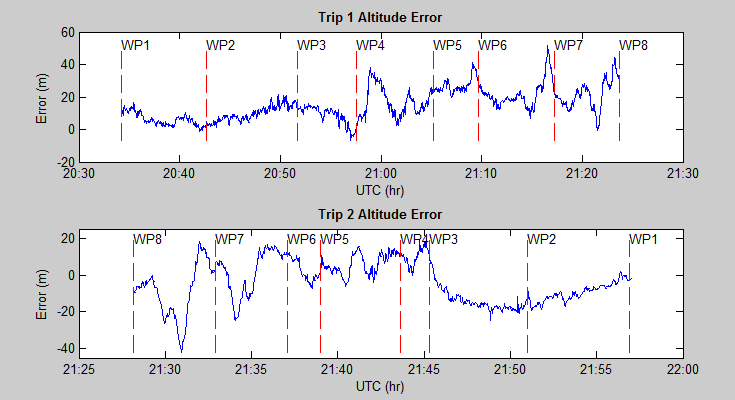
\includegraphics[width = 13cm]{AltitudeErr.PNG}
		\caption{Relative receiver altitude error observed during trips 1 and 2.}
		\label{fig:AltitudeErr}
	\end{figure}
	
	\section{Analysis}
	
	\noindent The error plots show that there was much greater relative error between the devices in the canyon than in the clear segment. An interesting artifact the authors found was that most of the waypoints where elevation measurements were taken did not show much error compared to the trip between them. The reason that most of the waypoints had more visibility, and less relative error, is most likely due to the condition of the canyon road. Much of the canyon had steep terrain with no shoulder or turn-off area, so stopping to perform elevation measurements at such places was nearly impossible.
		
	\vspace{5 mm}

	\noindent The route between waypoints 1 and 3 (clear segment) was in clear terrain, with waypoint 3 observing the most topographic elevation to the west at 20 degrees (see Appendix Figure~\ref{fig:AzElWaypoint3}). The authors considered waypoint 3 to be the entrance to the canyon, with the latter points being in the canyon (canyon segment). The data were first checked against a map of the road in Google Earth to ensure the data were close to the road, as hypothesized. Figure~\ref{fig:inboutClearSeg} shows a representative example for each trip in the clear segment; Figure~\ref{fig:GoodSignalStrength} shows a representative PRN signal strength in the clear segment.
	
	\begin{figure}[H]
		\centering
		\begin{subfigure}
			\centering
			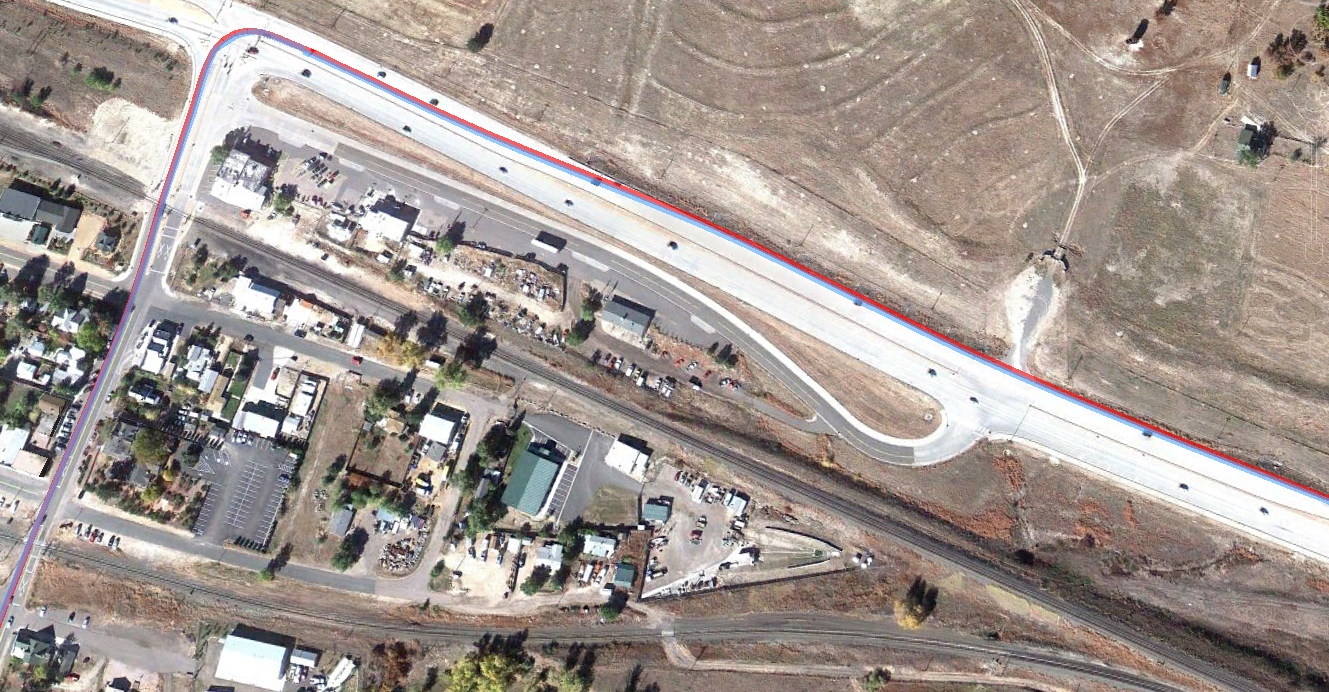
\includegraphics[width = 13cm]{inboutClearSeg.PNG}
		\end{subfigure}
		\begin{subfigure}
			\centering
			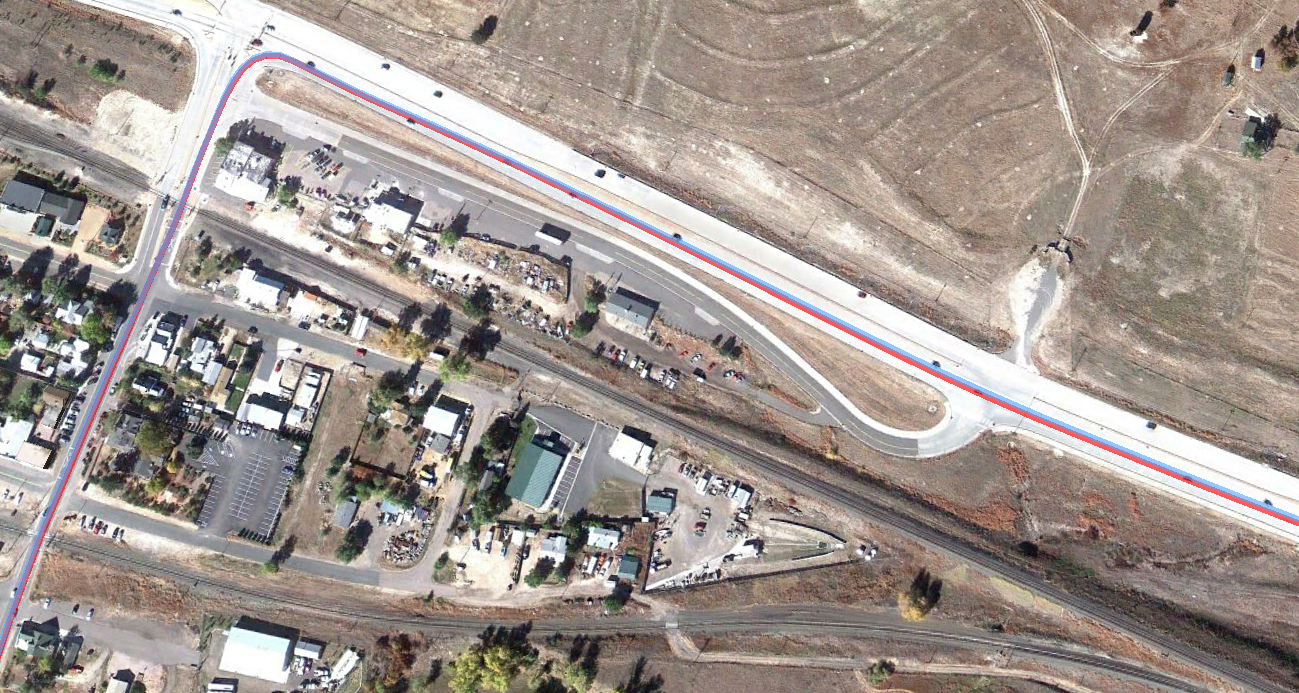
\includegraphics[width = 13cm]{outboutClearSeg.PNG}
		\end{subfigure}
		\caption{Representative examples of position accuracy in the clear segment. The colored lines are the path travelled.}
		\label{fig:inboutClearSeg}
	\end{figure}
	
	\noindent Clock synchronization between the receivers was initially a concern to the authors. The data were only recorded at integer-second intervals, which could produce a large error for a given epoch. This concern was abated when the clear segment's relative errors were analyzed. Between waypoints 1 and 2, the vehicle was traveling at 60 miles/hr ($\sim$27 m/s). A representative measurement from each receiver at the same time on the clear segment was taken to be 2.6 meters, as seen in Figure~\ref{fig:ClockError}. If the difference was completely due to clock biases, that difference would be ~0.1 s. However, pseudorange errors could be within this range of error, and the Garmin receiver had WAAS capability disabled. Thus, clock synchronization error was deemed low enough not to be an issue compared to other error sources, especially since the canyon segment had a top speed of 30 mph.
	
	\begin{figure}[H]
		\centering
		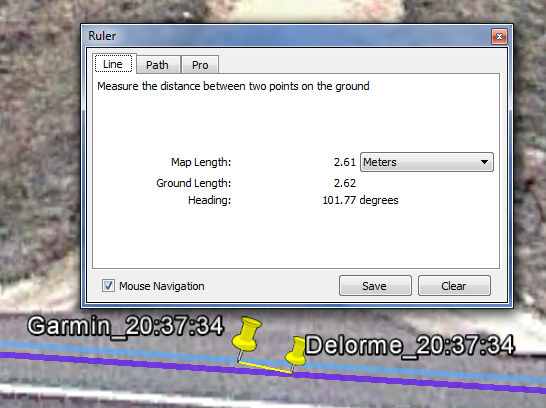
\includegraphics[width = 13cm]{ClockError.PNG}
		\caption{Difference in receiver positions with the same timestamps.}
		\label{fig:ClockError}
	\end{figure}
	
	\noindent Representative canyon data are visualized in Figure~\ref{fig:badPreWP4}. The purple line is track data from the Delorme receiver and the blue line is the track data from the Garmin receiver. The Delorme receiver, with WAAS enabled, stays close to the road in Google Earth. On the other hand, the receiver without WAAS on varies wildly throughout the canyon. Using Google's Street View capability, one can see that this magnitude of error happens when there is much less visibility of the sky. Appendix Figure~\ref{fig:AzElWaypoint4} shows the visibility plot near this location; Appendix Figure~\ref{fig:BadSignalStrength} shows a representative PRN signal strength.

	\begin{figure}[H]
		\centering
		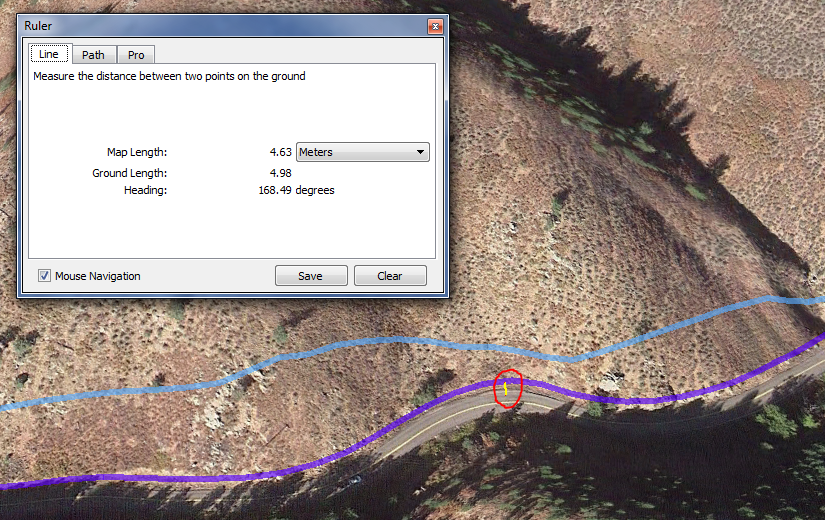
\includegraphics[width = 13cm]{badPreWP4.PNG}
		\caption{Representative example of position accuracy in the canyon segment. The purple line is the Delorme receiver, and the blue line is the Garmin receiver. }
		\label{fig:badPreWP4}
	\end{figure}

	\vspace{5 mm}
	
	\noindent The altitude difference between the receivers is more substantial than the latitude/longitude differences.  The error in the canyon segment is large, as expected. However, the altitude error varied by as much as 20 m in the clear segment, almost ten times that of the latitude and longitude relative errors.  Despite this large difference, the tracks were overlaid on the road quite well.  For this reason, the altitude was not further considered in the experiment, although it should be explored further.

	\section{Conclusion and Recommendations}
	
	\noindent The data from both trips, and both receivers, were unambiguous: GPS navigation was better with fewer topographic features, and worse in the canyon. With the WAAS enabled, the Delorme receiver was consistently closer to the road throughout the canyon segment. The Garmin, without WAAS, was much more error-prone. With these results, the hypothesis was confirmed. 
	
	\vspace{5 mm}
	
	\noindent The experiment could have benefited from more control in a few areas. Receivers of the same model and firmware versions would eliminate any potential differences between the performed position calculations. The receivers were also sitting on the dashboard of the car, which still had obstruction potential. Being able to set the receivers above the cabin would allow for maximal visibility (topography notwithstanding). An especially enterprising team could combine a camera system and accelerometers to constantly take pictures and measurements to be used in topographic elevation measurements throughout the route, instead of a few discrete points made at safe turn-offs.
	
	\vspace{5 mm}
	
	\noindent This experiment generated some questions the authors think could be explored. First, how accurate are the satellite images on Google Earth? They were assumed to be “truth” for the experiment, but error in the image placement would affect the perceived performance of the receivers. Additionally, are there survey data for the road that could be used to statistically fit the empirical data? This kind of analysis would yield more quantitative results than the use of Google Earth's ruler at various points. Finally, why were the height measurements so different between the receivers, compared to the latitude/longitude measurements?
	
	\vspace{5 mm}
	
	\noindent The experiment successfully demonstrated that open terrain allowed for better GPS receiver accuracy than terrain with much topographic masking. However, there were areas identified to improve its quality. The authors also recommend to explore the questions identified previously, as they may lead to more insight into the data. Qualitatively, both receivers appeared to perform well in the canyon, despite the reduced satellite visibility. Even the Garmin with WAAS disabled could perform crude navigation of the canyon if needed, although it would not do well for precision applications. The experiment should be repeated in an area with higher, and more consistent, topographic features to further mask visibility and potentially draw sharper conclusions.
	
	
	\begin{thebibliography}{9}% maximum number of references (for label width)
		\bibitem{Misra:2012} 
		\noindent Misra, P. and Enge, P. \emph{Global Positioning System Signals, Measurements and Performance Revised Second Edition}, Ganga-Jamuna Press, 2012.
		
		
	\end{thebibliography}
	
	\newpage

	\section{Appendix}
	\noindent This appendix contains supplemental pictures to further support the conclusions drawn previously.  Figs. ~\ref{fig:GoodSignalStrength} and ~\ref{fig:BadSignalStrength}. Figs ~\ref{fig:AzElWaypoint1} -~\ref{fig:AzElWaypoint8} show the elevation mask on sky visibility plots.
	
	\begin{figure}[H]
		\centering
		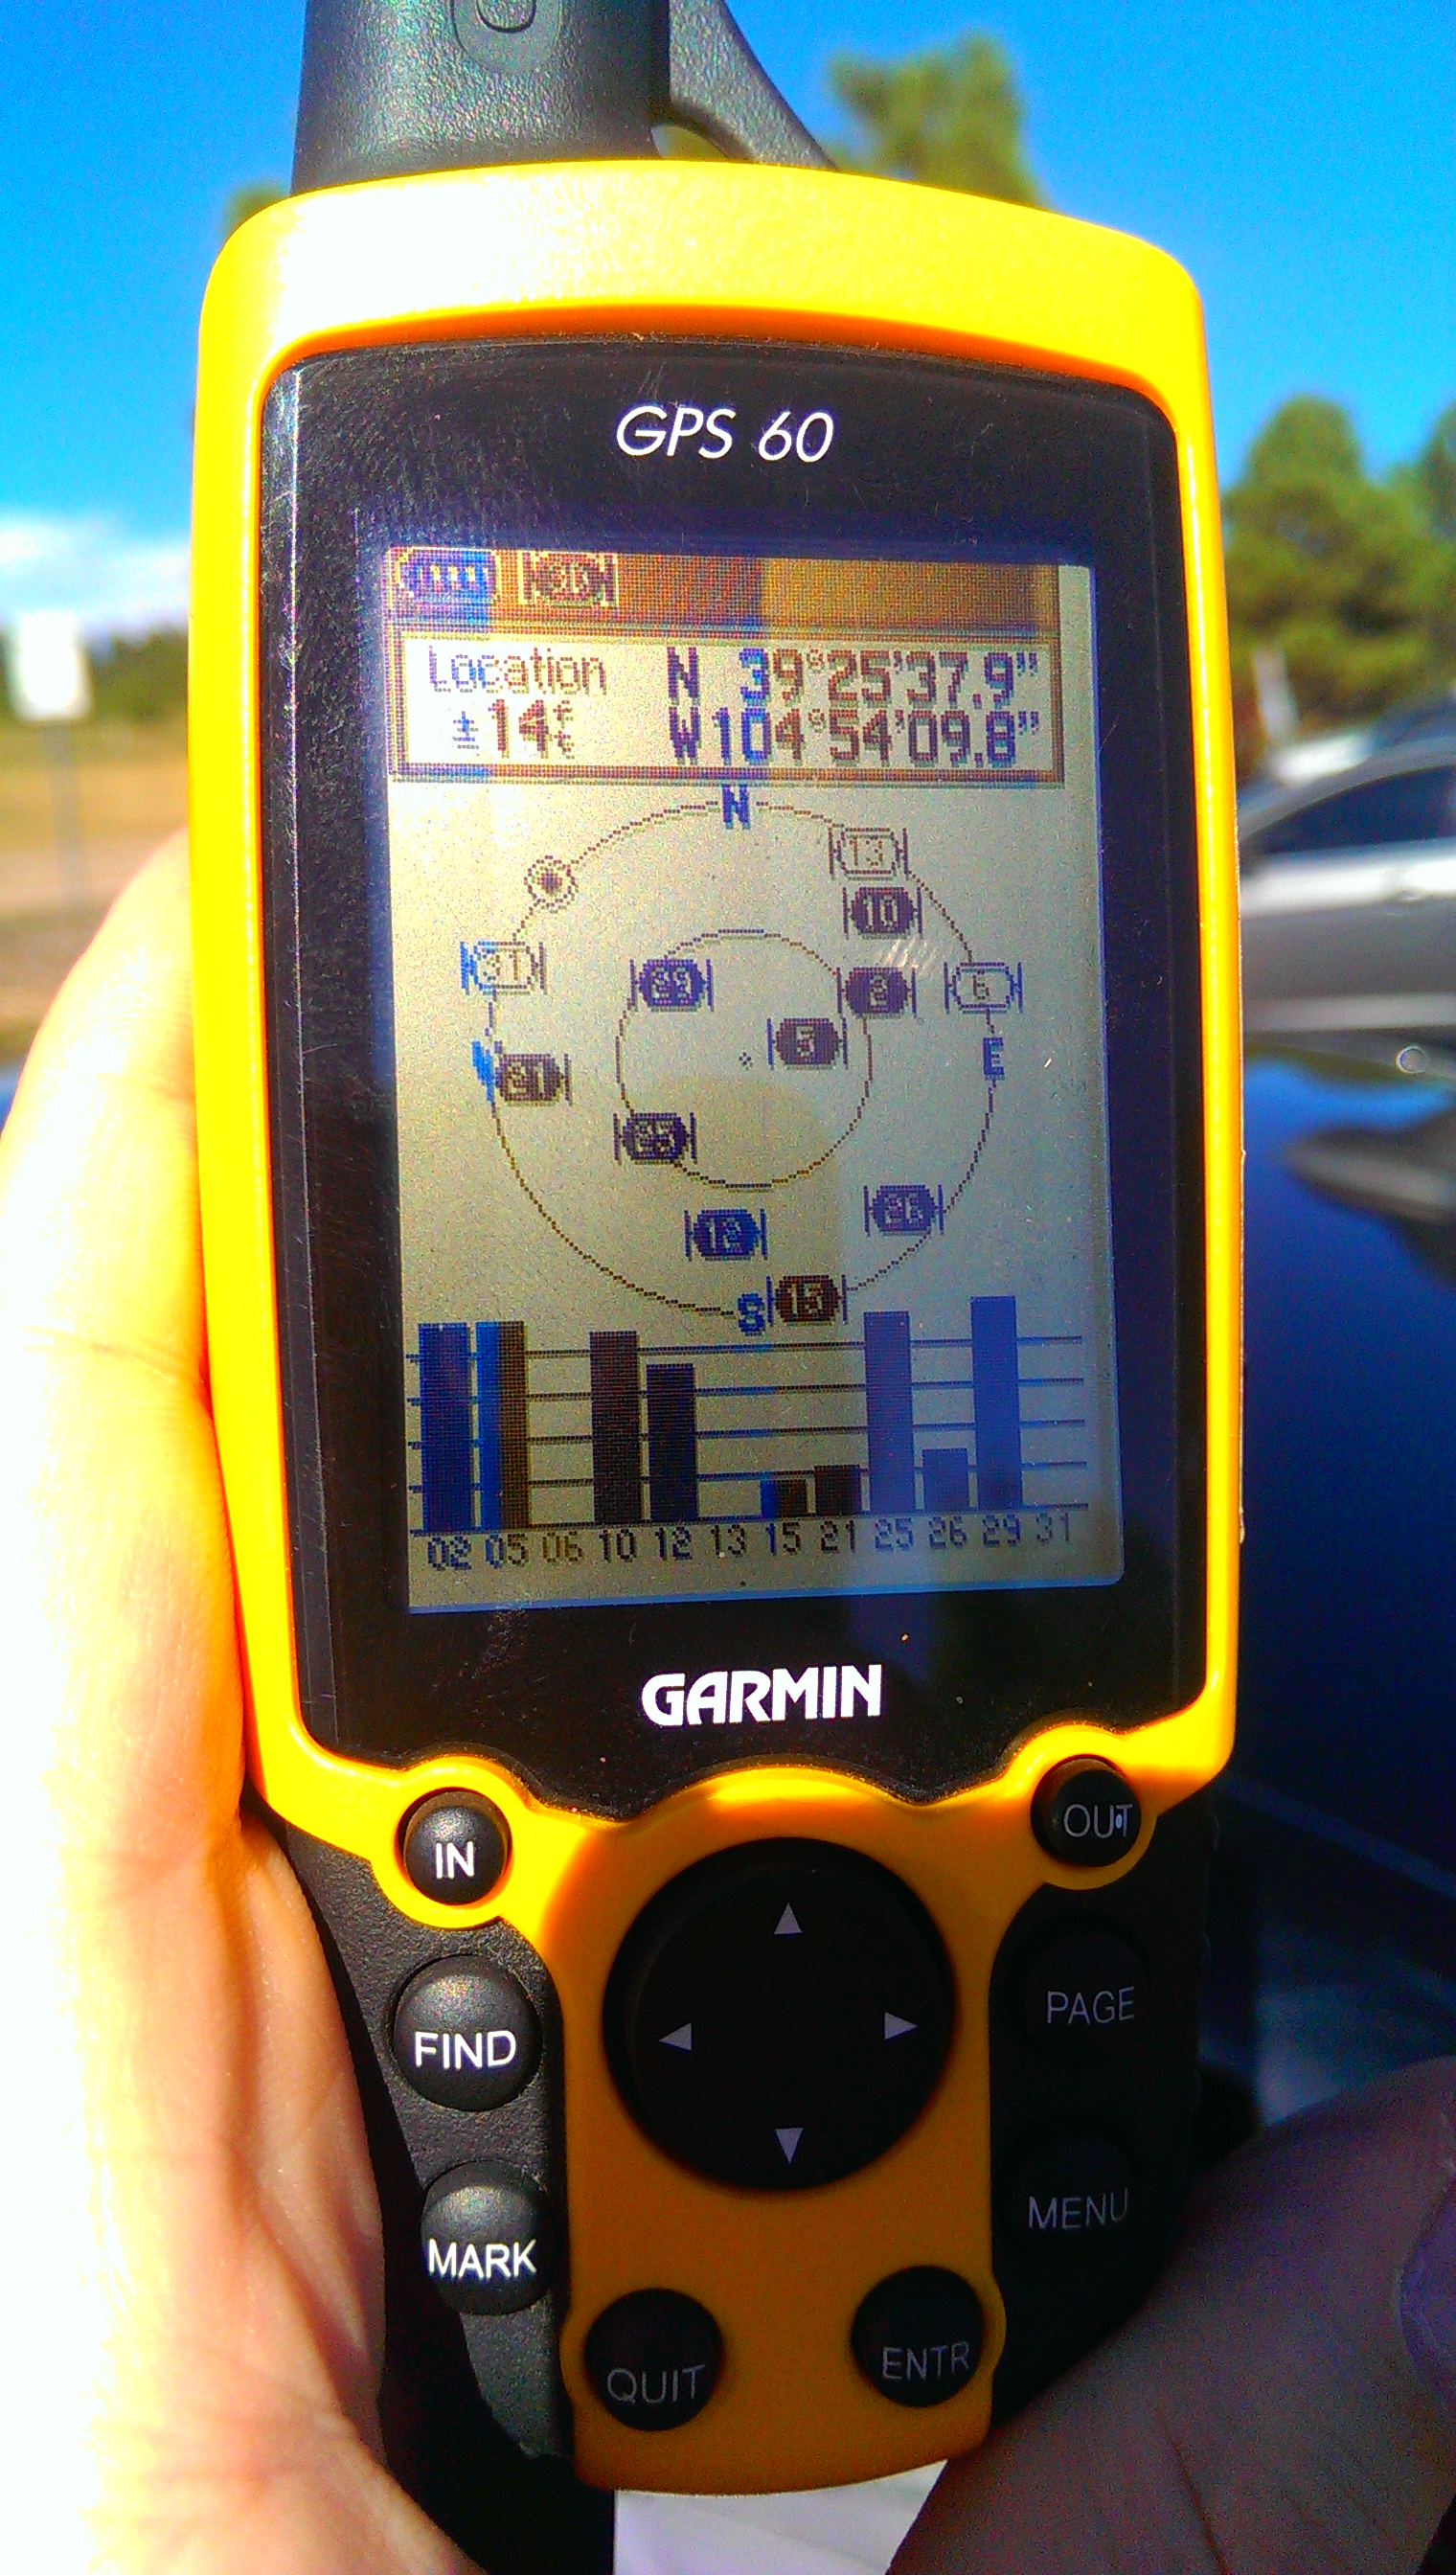
\includegraphics[width = 10cm]{GoodSignalStrength.jpg}
		\caption{Representative example of PRN signal strength in the clear segment.}
		\label{fig:GoodSignalStrength}
	\end{figure}
		
	\begin{figure}[H]
		\centering
		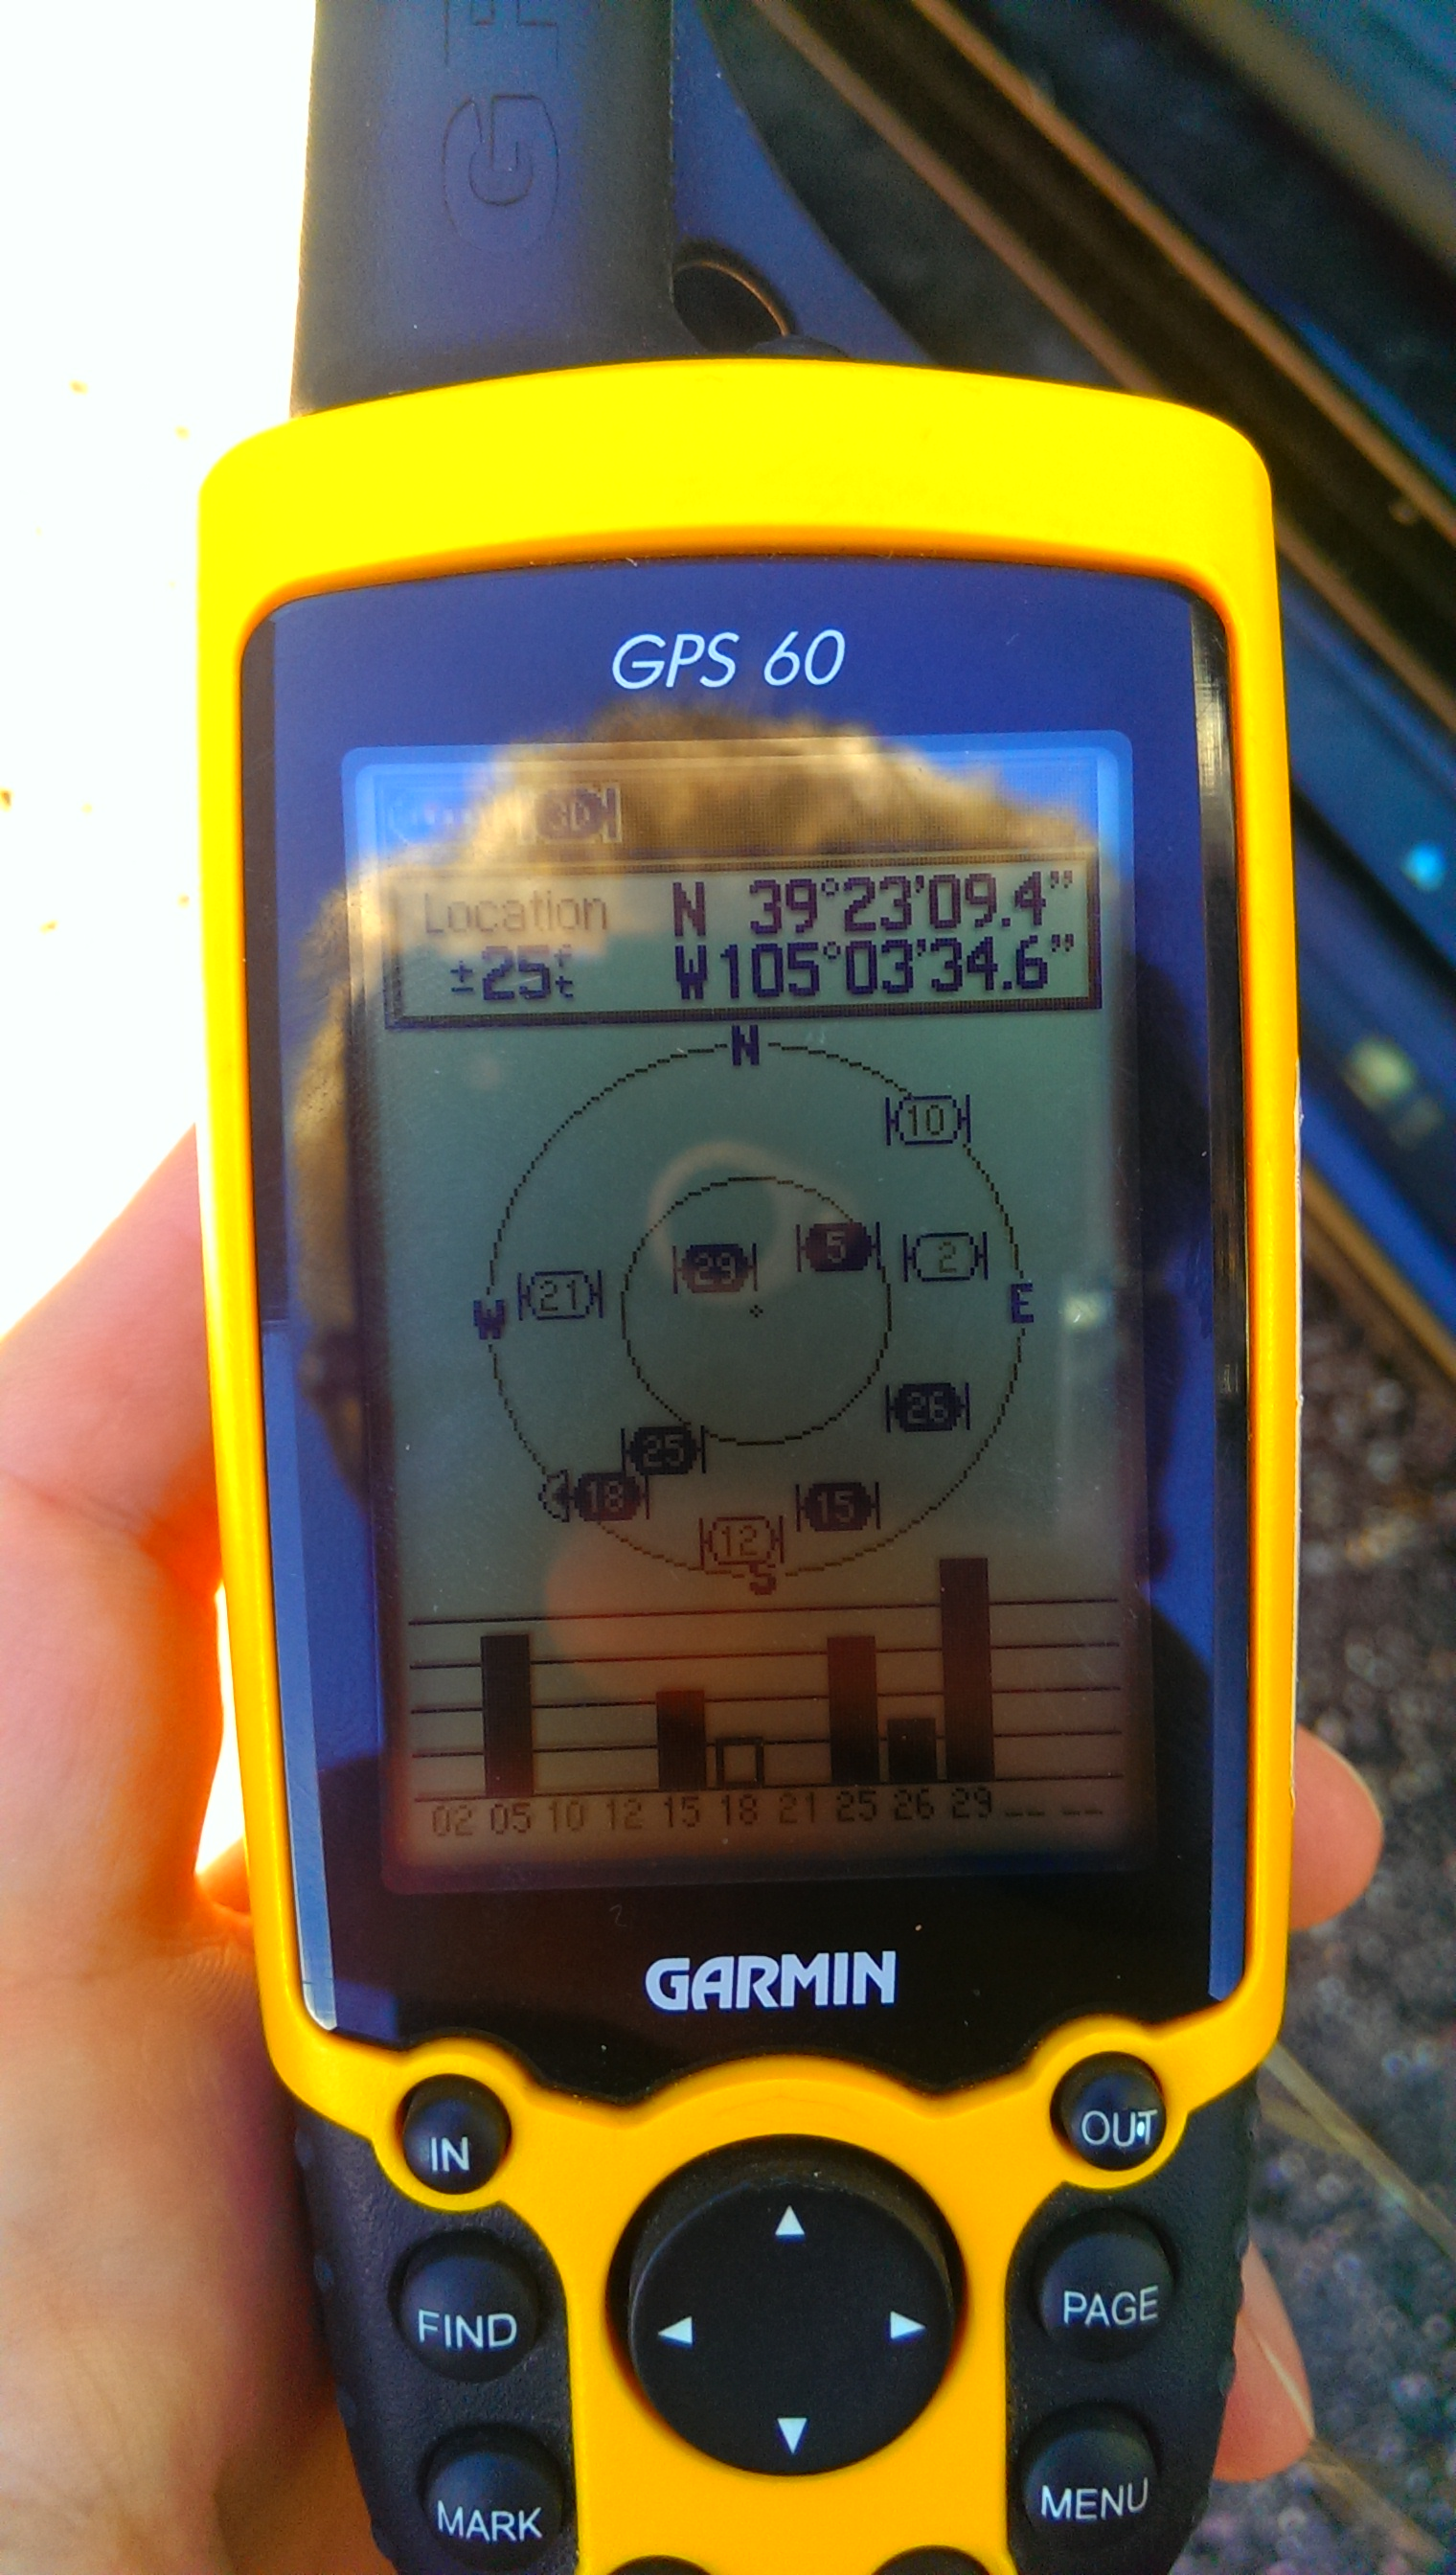
\includegraphics[width = 10cm]{BadSignalStrength.jpg}
		\caption{Representative example of PRN signal strength in the canyon segment. }
		\label{fig:BadSignalStrength}
	\end{figure}
	
	\begin{figure}[H]
		\centering
		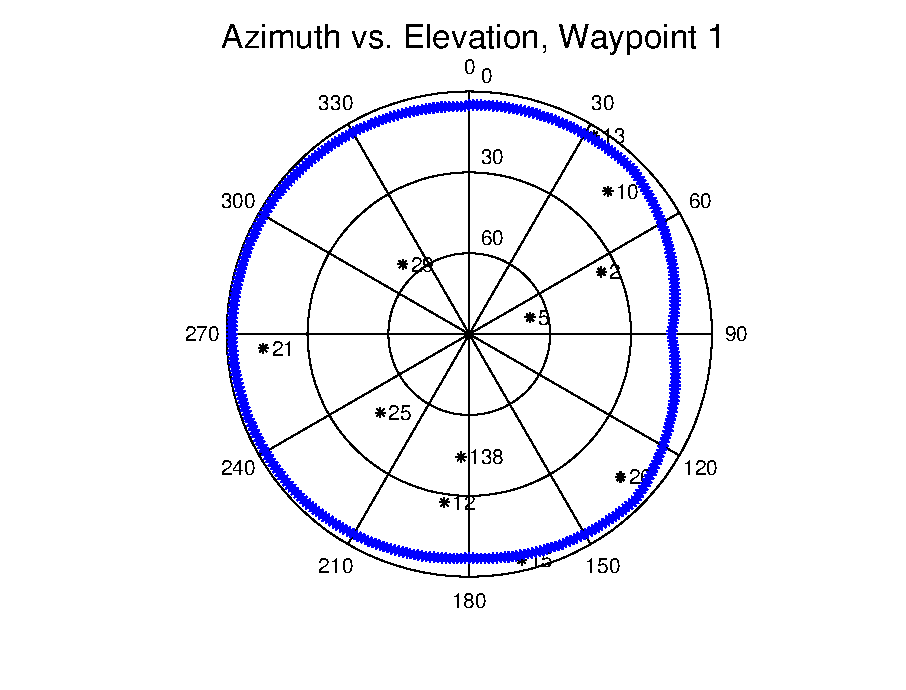
\includegraphics[width = 13cm]{AzElWaypoint1.eps}
		\caption{Plot for horizon mask for Waypoint 1. Time = 10/04/2014 20:30:26 UTC}
		\label{fig:AzElWaypoint1}
	\end{figure}
		
	\begin{figure}[H]
		\centering
		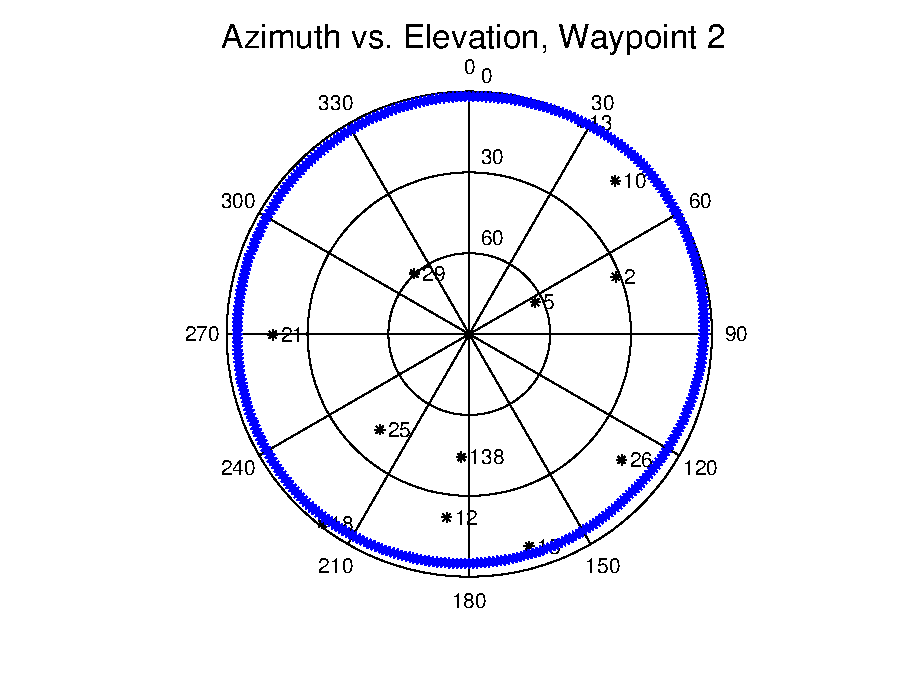
\includegraphics[width = 13cm]{AzElWaypoint2.eps}
		\caption{Plot for horizon mask for Waypoint 2. Time = 10/04/2014 20:42:35 UTC}
		\label{fig:AzElWaypoint2}
	\end{figure}
	
	\begin{figure}[H]
		\centering
		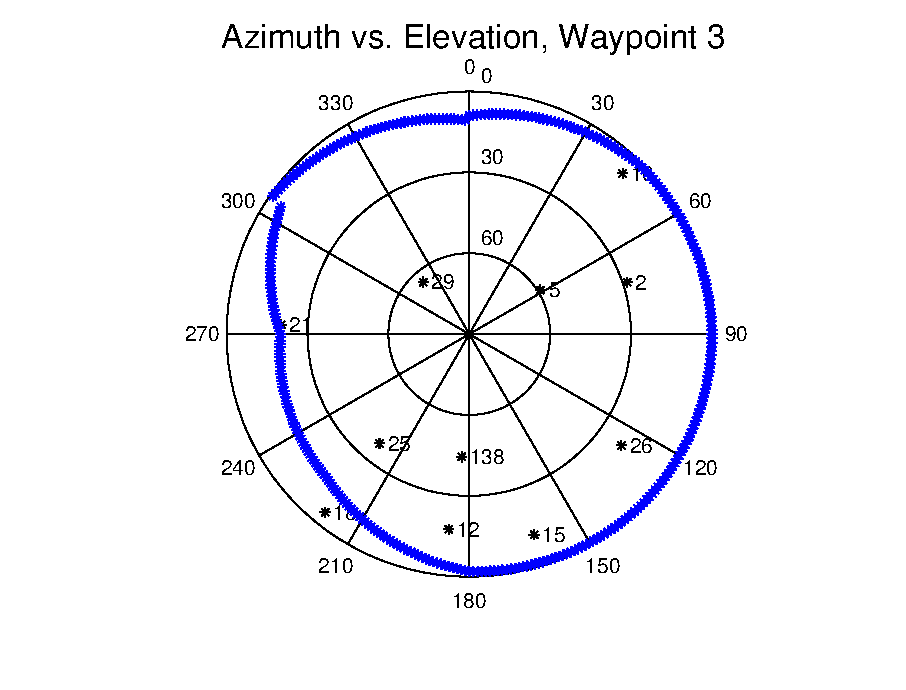
\includegraphics[width = 13cm]{AzElWaypoint3.eps}
		\caption{Plot for horizon mask for Waypoint 3. Time = 10/04/2014 20:52:34 UTC}
		\label{fig:AzElWaypoint3}
	\end{figure}
	
	\begin{figure}[H]
		\centering
		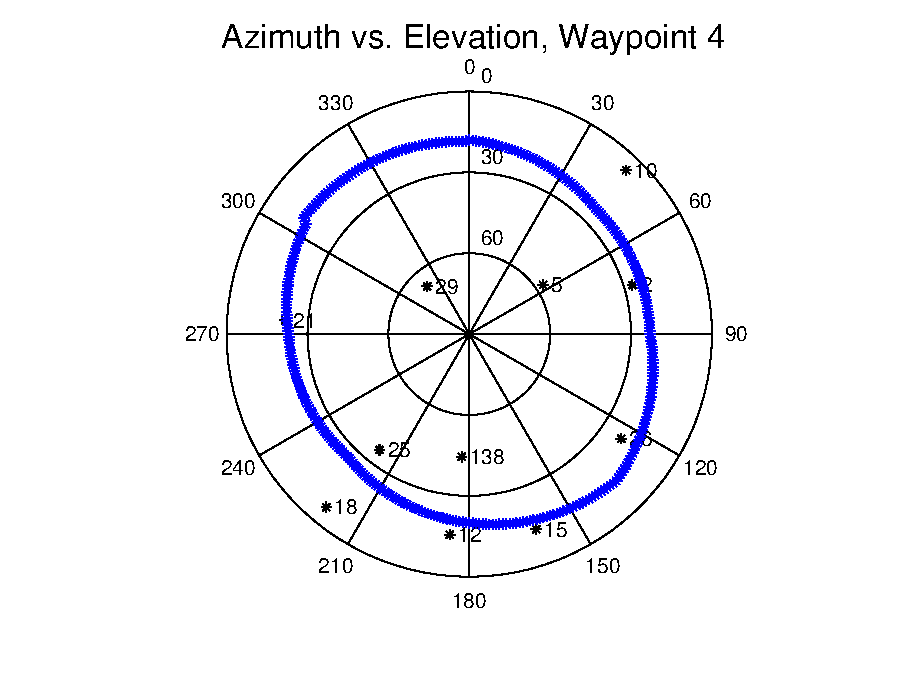
\includegraphics[width = 13cm]{AzElWaypoint4.eps}
		\caption{Plot for horizon mask for Waypoint 4. Time = 10/04/2014 20:57:07 UTC}
		\label{fig:AzElWaypoint4}
	\end{figure}
	
	\begin{figure}[H]
		\centering
		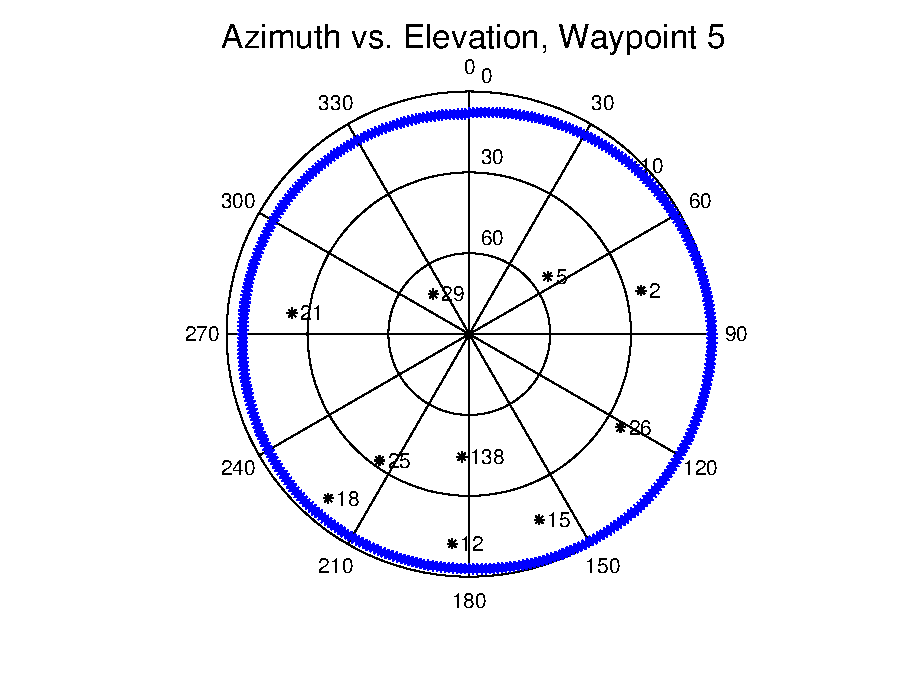
\includegraphics[width = 13cm]{AzElWaypoint5.eps}
		\caption{Plot for horizon mask for Waypoint 5. Time = 10/04/2014 21:04:55 UTC}
		\label{fig:AzElWaypoint5}
	\end{figure}
	
	\begin{figure}[H]
		\centering
		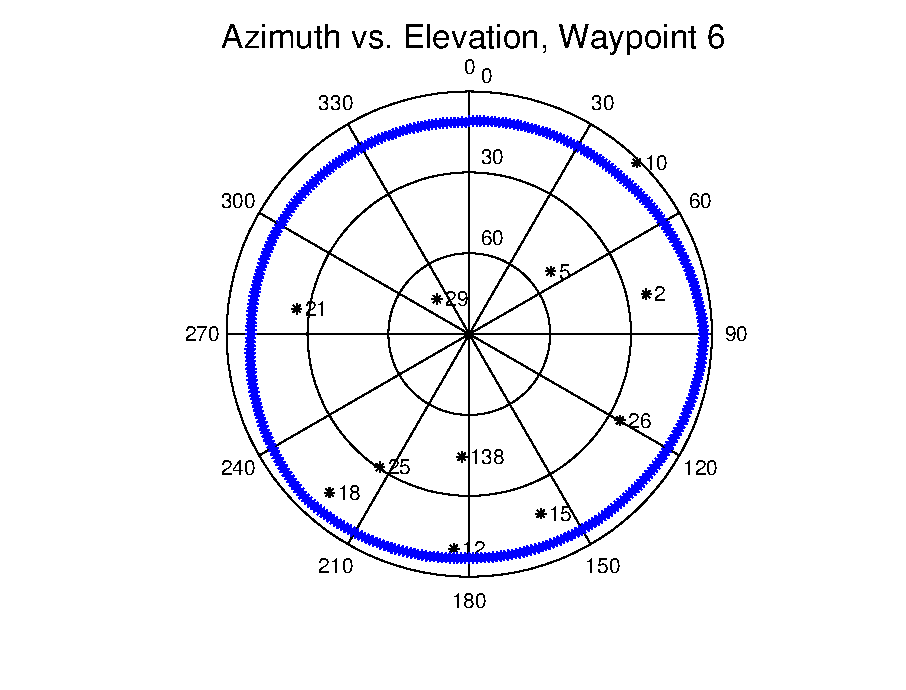
\includegraphics[width = 13cm]{AzElWaypoint6.eps}
		\caption{Plot for horizon mask for Waypoint 6. Time = 10/04/2014 21:09:40 UTC}
		\label{fig:AzElWaypoint6}
	\end{figure}
	
	\begin{figure}[H]
		\centering
		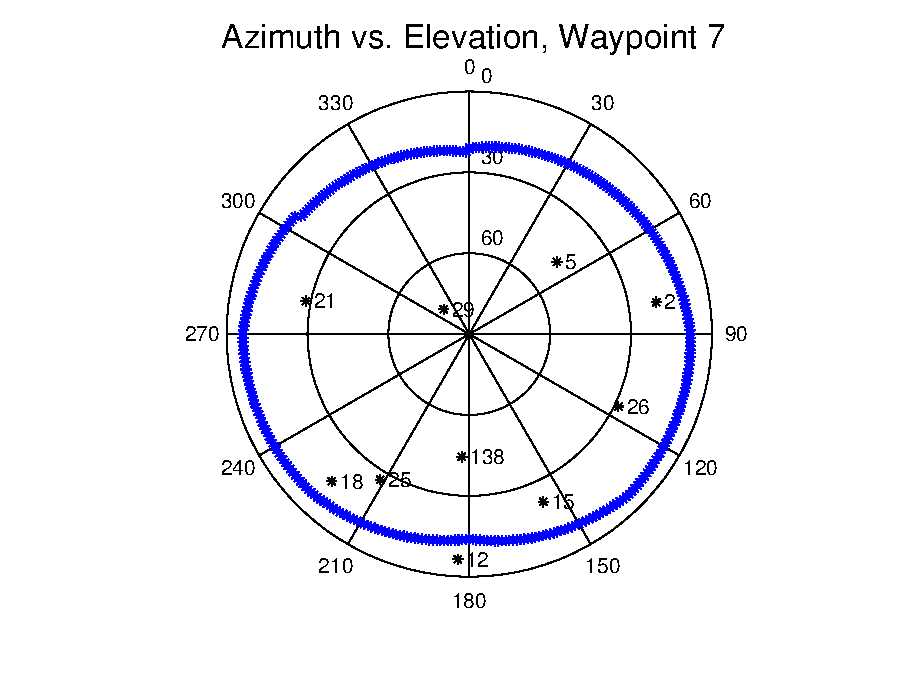
\includegraphics[width = 13cm]{AzElWaypoint7.eps}
		\caption{Plot for horizon mask for Waypoint 7. Time = 10/04/2014 21:19:07 UTC}
		\label{fig:AzElWaypoint7}
	\end{figure}
	
	\begin{figure}[H]
		\centering
		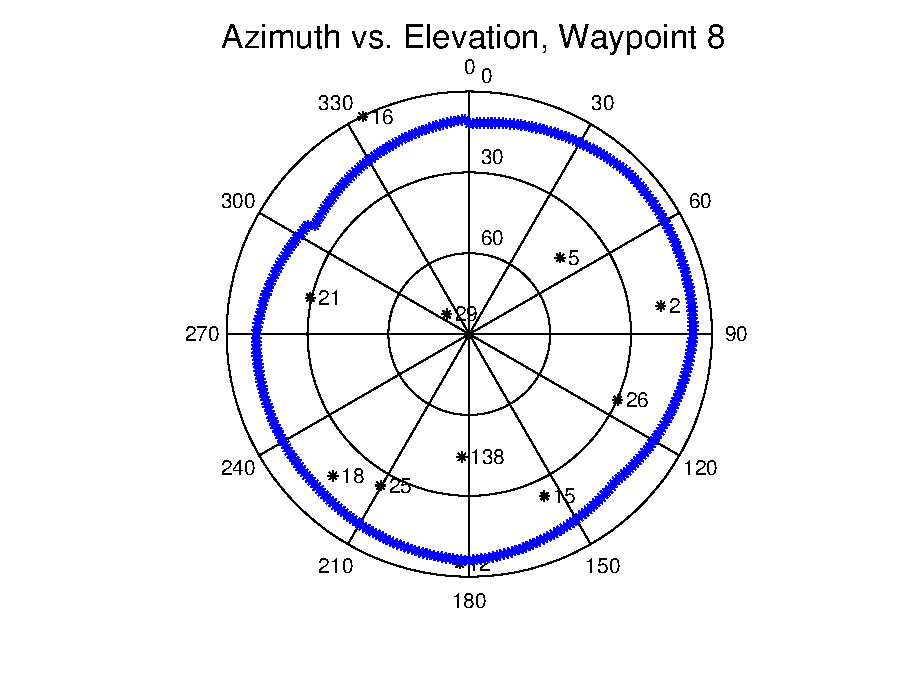
\includegraphics[width = 13cm]{AzElWaypoint8.eps}
		\caption{Plot for horizon mask for Waypoint 8. Time = 10/04/2014 21:23:29 UTC}
		\label{fig:AzElWaypoint8}
	\end{figure}
	
%    \section{Appendix B}
%This appendix contains all Matlab code used by the authors to analyize their data.
%    
%    \lstset{language=Matlab,%
%    	%basicstyle=\color{red},
%    	breaklines=true,%
%    	morekeywords={matlab2tikz},
%    	keywordstyle=\color{blue},%
%    	morekeywords=[2]{1}, keywordstyle=[2]{\color{black}},
%    	identifierstyle=\color{black},%
%    	stringstyle=\color{mylilas},
%    	commentstyle=\color{mygreen},%
%    	showstringspaces=false,%without this there will be a symbol in the places where there is a space
%    	numbers=left,%
%    	numberstyle={\tiny \color{black}},% size of the numbers
%    	numbersep=9pt, % this defines how far the numbers are from the text
%    	emph=[1]{for,end,break},emphstyle=[1]\color{red}, %some words to emphasise
%    	%emph=[2]{word1,word2}, emphstyle=[2]{style},   
%    }
    
%    \lstinputlisting{ASEN5090_ecef2azelrange.m}
%    \vspace{5mm}
%    
%    \lstinputlisting{ASEN5090_GPSvis.m}
%    \vspace{5mm}
%\lstinputlisting{HW5_rel_err.m}
%\vspace{5mm}
%\lstinputlisting{import_gps_data.m}
%\vspace{5mm}
%\lstinputlisting{datenum8601.m}
%\vspace{5mm}
%\lstinputlisting{lab_err_plots.m}
%\vspace{5mm}
	
\end{document}

% - Release $Name:  $ -
